\documentclass[tikz,border=10pt]{standalone}
\usepackage{tikz}

\begin{document}
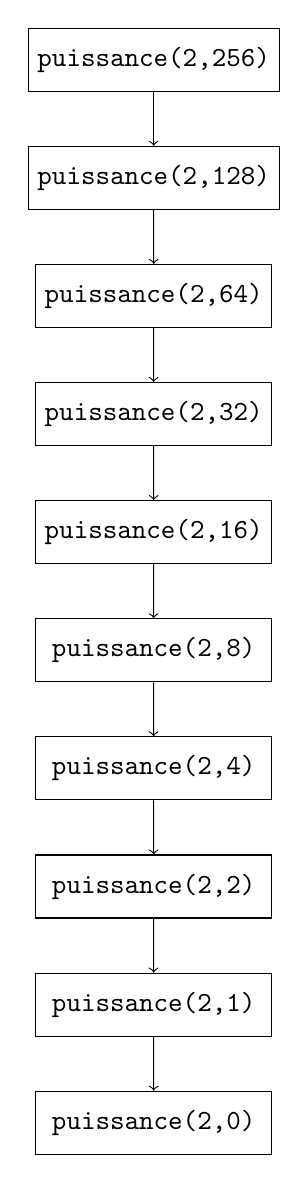
\begin{tikzpicture}[
  node/.style={rectangle,draw,minimum width=3cm,minimum height=8mm,align=center},
  level distance=15mm,
  sibling distance=20mm,
  edge from parent/.style={draw,->} % <-- flèches
]

\node[node] {\texttt{puissance(2,256)}}
  child {node[node] {\texttt{puissance(2,128)}}
    child {node[node] {\texttt{puissance(2,64)}}
      child {node[node] {\texttt{puissance(2,32)}}
        child {node[node] {\texttt{puissance(2,16)}}
          child {node[node] {\texttt{puissance(2,8)}}
            child {node[node] {\texttt{puissance(2,4)}}
              child {node[node] {\texttt{puissance(2,2)}}
                child {node[node] {\texttt{puissance(2,1)}}
                 child {node[node] {\texttt{puissance(2,0)}}}
}}}}}}}};

\end{tikzpicture}
\end{document}
